\documentclass[11pt]{article}
\usepackage[margin=1in]{geometry}
\usepackage{amsmath,amssymb,amsthm,mathtools}
\usepackage{graphicx}
\usepackage[hidelinks]{hyperref}
\usepackage{microtype}

\newtheorem{theorem}{Theorem}
\newtheorem{lemma}{Lemma}
\newcommand{\R}{\mathbb R}
\newcommand{\norm}[1]{\left\lVert#1\right\rVert}
\newcommand{\Sym}{\operatorname{Sym}}
\newcommand{\ran}{\operatorname{ran}}

\title{A scalar first-order necessity theorem for limiting Sobolev
inequalities on stratified groups}
\author{Candidate partial result for arXiv:2007.14532}
\date{11 August 2026}

\begin{document}
\maketitle

\begin{center}
\fbox{\parbox{0.91\textwidth}{\textbf{Status.}
Candidate partial result, likely valid, pending human review.  The result
settles the source question only for scalar first-order operators.}}
\end{center}

\section{Source question}

Van Schaftingen and Yung study a stratified homogeneous group $G$ with first
layer $\mathfrak g_1$, homogeneous dimension $Q$, and a homogeneous
left-invariant operator $A(D)$ of order $k$.  Their endpoint estimate is
\begin{equation}\label{eq:endpoint-general}
 \norm{D^{k-1}u}_{L^{Q/(Q-1)}(G;V)}
 \le C\norm{A(D)u}_{L^1(G;E)},\qquad u\in C_c^\infty(G;V).
\end{equation}
They prove it from (i) maximal hypoellipticity and (ii) the existence of a
compatible homogeneous operator $L(D)$ whose symmetrization is cocanceling
\cite{VSY}.  On PDF page 4 they ask whether validity of
\eqref{eq:endpoint-general} implies these conditions on a general stratified
homogeneous group.

The three source crops below give equation (1.7), conditions (i)--(ii), and
the open-question paragraph, respectively.

\begin{figure}[ht]
  \centering
  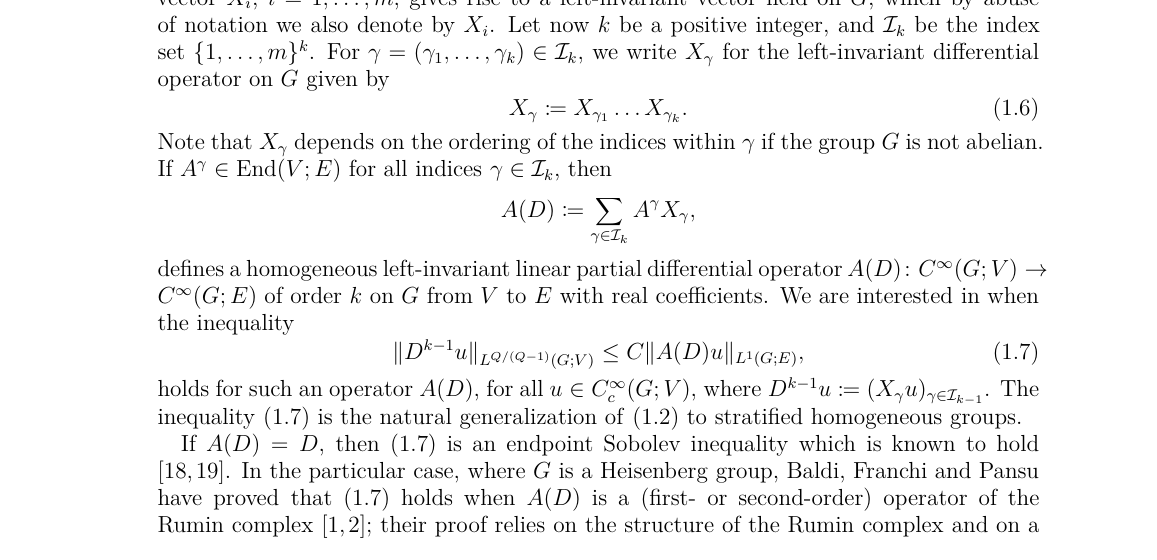
\includegraphics[width=\textwidth]{figures/inequality_1_7_crop.png}
  \caption{The endpoint estimate (1.7), source PDF page 2.}
\end{figure}

\begin{figure}[ht]
  \centering
  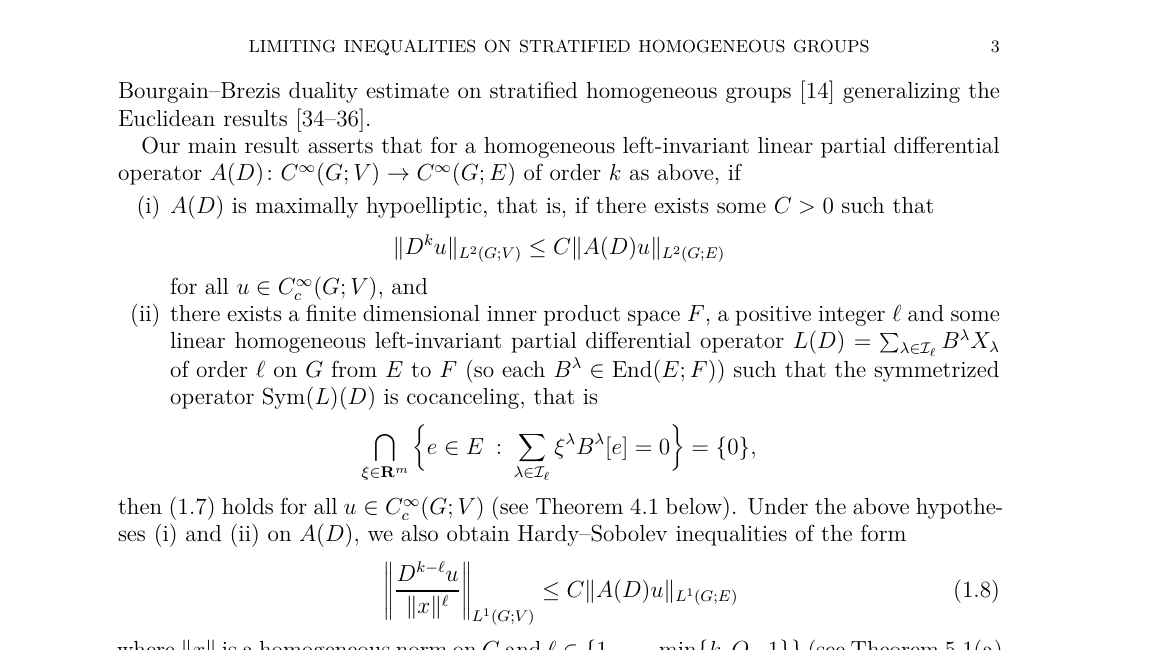
\includegraphics[width=\textwidth]{figures/conditions_crop.png}
  \caption{The sufficient conditions (i)--(ii), source PDF page 3.}
\end{figure}

\begin{figure}[ht]
  \centering
  
\includegraphics[width=\textwidth]{figures/open_problem_crop.png}
  \caption{The open question, source PDF page 4.}
\end{figure}

\clearpage
\section{Definitions and scope}

Write
\[
 \mathfrak g=\mathfrak g_1\oplus\cdots\oplus\mathfrak g_r,
 \qquad [\mathfrak g_i,\mathfrak g_j]\subseteq\mathfrak g_{i+j},
 \qquad Q=\sum_{j=1}^r j\dim\mathfrak g_j,
\]
and let $X_1,\ldots,X_m$ be a basis of $\mathfrak g_1$.  We assume $Q\ge2$.
For a finite-dimensional inner-product space $E$ and a linear map
$T:\R^m\to E$, define the scalar first-order operator
\begin{equation}\label{eq:AT}
 A_T(D)u=T(Du)=T(X_1u,\ldots,X_mu).
\end{equation}
If $L(D)$ is a homogeneous left-invariant operator from $E$ to another
finite-dimensional space, it is \emph{compatible} with $A_T(D)$ when
$L(D)A_T(D)=0$.  Its symmetrization is \emph{cocanceling} when
\[
 \bigcap_{\xi\in\R^m}\ker\Sym(L)(\xi)=\{0\}.
\]

\section{Proof intuition}

Suppose $T$ loses a horizontal direction.  Choose that direction as $X_1$.
Take a test function that remains compact in the $x_1$ coordinate, while all
other exponential coordinates are expanded according to their homogeneous
weights.  The transverse volume is $R^{Q-1}$.  The leading $X_1$ derivative
is killed by $T$, and every derivative falling on the transverse cutoff costs
$R^{-1}$.  Consequently the right side of the endpoint estimate is only
$O(R^{Q-2})$.  The left side is of order
$R^{(Q-1)/q}=R^{Q-2+1/Q}$ for $q=Q/(Q-1)$, giving a contradiction.

Thus $T$ is injective.  This already gives maximal hypoellipticity, since a
finite-dimensional injective map is bounded below.  For compatibility, use
the source paper's explicit compatible cocanceling operator for the full
horizontal gradient, transport it to $\ran T$ through a left inverse, and add
a pure-derivative block on a complement of $\ran T$.

The argument does not address $k\ge2$ or $\dim V>1$.

\section{The partial theorem}

\begin{theorem}[Scalar first-order characterization]\label{thm:main}
Let $G$ be a stratified homogeneous group with homogeneous dimension $Q\ge2$,
let $E$ be finite-dimensional, and let $A_T(D)$ be given by
\eqref{eq:AT}.  Put $q=Q/(Q-1)$.  The following are equivalent.
\begin{enumerate}
\item There exists $C<\infty$ such that
\begin{equation}\label{eq:endpoint}
 \norm{u}_{L^q(G)}\le C\norm{A_T(D)u}_{L^1(G;E)}
 \quad\text{for all }u\in C_c^\infty(G).
\end{equation}
\item The coefficient map $T:\R^m\to E$ is injective.
\item The operator $A_T(D)$ is maximally hypoelliptic and admits a compatible
homogeneous $L(D)$ such that $\Sym(L)(D)$ is cocanceling.
\end{enumerate}
In particular, the source question has an affirmative answer throughout the
scalar first-order class.
\end{theorem}

\begin{proof}
We first prove $(1)\Rightarrow(2)$, which is the new necessity argument.
Suppose instead that $0\ne c\in\ker T$.  Change the basis of
$\mathfrak g_1$ so that $X_1=c$.  This only changes the equivalent norm used
for $Du$.  In the corresponding coordinates, $T(e_1)=0$.

Complete $X_1,\ldots,X_m$ to a homogeneous basis
$Y_1=X_1,Y_2=X_2,\ldots,Y_N$ of $\mathfrak g$, and let $w_\nu$ be the
homogeneous weight of $Y_\nu$.  Thus $w_1=\cdots=w_m=1$ and
$\sum_{\nu=1}^Nw_\nu=Q$.  Use exponential coordinates of the first kind
\[
 (x_1,\ldots,x_N)\longmapsto
 \exp\left(\sum_{\nu=1}^Nx_\nu Y_\nu\right).
\]
Haar measure is a constant multiple of Lebesgue measure in these coordinates.
The horizontal left-invariant fields have the standard polynomial form
\begin{equation}\label{eq:poly-fields}
 X_j=\partial_{x_j}+
 \sum_{\nu:m<\nu\le N}p_{j\nu}(x)\partial_{x_\nu},
\end{equation}
where $p_{j\nu}$ is a polynomial homogeneous of weighted degree
$w_\nu-1$.

Choose nonzero $\phi\in C_c^\infty(\R)$ and nonzero
$\eta\in C_c^\infty(\R^{N-1})$.  For $R\ge1$, set
\begin{align*}
 \eta_R(x_2,\ldots,x_N)
  &=\eta(R^{-w_2}x_2,\ldots,R^{-w_N}x_N),\\
 u_R(x)&=\phi(x_1)\eta_R(x_2,\ldots,x_N).
\end{align*}
These are admissible compactly supported smooth functions.  A change of
variables gives
\begin{equation}\label{eq:left-growth}
 \norm{u_R}_{L^q(G)}
 =c_{\phi,\eta}R^{(Q-1)/q}
 =c_{\phi,\eta}R^{Q-2+1/Q}.
\end{equation}

We claim that, uniformly on $\operatorname{supp}\phi\times
\operatorname{supp}\eta_R$,
\begin{equation}\label{eq:cutoff-derivative}
 |X_j\eta_R|\le \frac{C}{R},\qquad j=1,\ldots,m.
\end{equation}
The direct derivative $\partial_{x_j}\eta_R$ has this bound (and it is zero
for $j=1$).  For a monomial $x^\alpha$ in $p_{j\nu}$, weighted homogeneity
gives
\[
 \sum_{\mu=1}^Nw_\mu\alpha_\mu=w_\nu-1.
\]
The coordinate $x_1$ stays in a fixed compact set, while
$|x_\mu|=O(R^{w_\mu})$ for $\mu\ge2$.  Hence
\[
 |x^\alpha|=O\left(
 R^{\sum_{\mu\ge2}w_\mu\alpha_\mu}\right)
 =O(R^{w_\nu-1-\alpha_1}).
\]
Multiplication by
$\partial_{x_\nu}\eta_R=O(R^{-w_\nu})$ gives $O(R^{-1-\alpha_1})$,
and therefore \eqref{eq:cutoff-derivative} follows from
\eqref{eq:poly-fields}.

Since $X_jx_1=\delta_{j1}$ and $T(e_1)=0$,
\begin{align*}
 A_T(D)u_R
 &=T(e_1)\phi'(x_1)\eta_R
   +\phi(x_1)\sum_{j=1}^mT(e_j)X_j\eta_R\\
 &=\phi(x_1)\sum_{j=1}^mT(e_j)X_j\eta_R.
\end{align*}
The support has measure $O(R^{Q-1})$, so
\begin{equation}\label{eq:right-growth}
 \norm{A_T(D)u_R}_{L^1(G;E)}\le CR^{Q-2}.
\end{equation}
Combining \eqref{eq:left-growth}, \eqref{eq:right-growth}, and
\eqref{eq:endpoint} would give $R^{1/Q}\le C'$ for every $R\ge1$, a
contradiction.  Thus $T$ is injective.

Next assume (2).  Since $T$ is an injective map between finite-dimensional
spaces, there is $c>0$ such that $|Tv|\ge c|v|$.  Therefore
\begin{equation}\label{eq:maxhyp}
 \norm{Du}_{L^2(G)}\le c^{-1}\norm{A_T(D)u}_{L^2(G;E)},
\end{equation}
so $A_T(D)$ is maximally hypoelliptic.  The endpoint inequality also follows
directly from the horizontal Sobolev inequality (Proposition 7.1 of
\cite{VSY}):
\[
 \norm{u}_{L^q(G)}\le C_G\norm{Du}_{L^1(G)}
 \le C_Gc^{-1}\norm{A_T(D)u}_{L^1(G;E)}.
\]

It remains to verify the compatibility part of (3).  Proposition 7.1 of
\cite{VSY} constructs a homogeneous operator
\[
 L_\nabla(D):C^\infty(G;\R^m)\longrightarrow C^\infty(G;F_0)
\]
of some order $s$ (their construction gives $s=r+1$) such that
\begin{equation}\label{eq:source-L}
 L_\nabla(D)D=0,
 \qquad
 \bigcap_{\xi\in\R^m}\ker\Sym(L_\nabla)(\xi)=\{0\}.
\end{equation}
Let $E_0=\ran T$, choose a complement $E_1$ with $E=E_0\oplus E_1$, let
$P:E\to E_0$ be the associated projection, and let $S:E\to\R^m$ equal
$T^{-1}$ on $E_0$ and zero on $E_1$.  Define an order-$s$ operator on $E_1$
by
\[
 H(D)h=(X_1^sh,\ldots,X_m^sh).
\]
Finally set
\begin{equation}\label{eq:block-L}
 L(D)f=\bigl(L_\nabla(D)Sf,\ H(D)(I-P)f\bigr).
\end{equation}
It is homogeneous of order $s$, and \eqref{eq:source-L} gives
\[
 L(D)A_T(D)u
 =\bigl(L_\nabla(D)Du,0\bigr)=0.
\]
If $e=e_0+e_1\in E_0\oplus E_1$ lies in
$\ker\Sym(L)(\xi)$ for every $\xi$, the first block and
\eqref{eq:source-L} give $Se_0=0$, hence $e_0=0$.  The second block has
symbol
\[
 \Sym(H)(\xi)e_1=(\xi_1^se_1,\ldots,\xi_m^se_1),
\]
whose common kernel is zero, so $e_1=0$.  Thus $\Sym(L)$ is cocanceling and
(2) implies (3).  Finally, (3) implies (1) by the source paper's main
endpoint theorem \cite[Theorem 4.1]{VSY}.  This completes the equivalence.
\end{proof}

\section{Verification and limitations}

The exponent gap is strict:
\[
 \frac{Q-1}{Q/(Q-1)}-(Q-2)=\frac1Q>0.
\]
The proof uses no numerical or symbolic computation.  The main review point
is the standard polynomial form \eqref{eq:poly-fields} and its use under the
partial dilation; the monomial calculation above makes the required uniform
bound explicit.

The theorem assumes scalar domain $V=\R$, order $k=1$, and $Q\ge2$.  The
source question remains open here for higher order and for vector-valued
domains.  In those cases, a kernel of the representation symbol need not
reduce to a single missing weight-one coordinate, so the present transverse
cutoff does not settle the Rockland condition.

\section{Novelty check}

A bounded check was performed on 11 August 2026 using the run's registry,
solution, attempt, and proof-gap indexes; the locally loaded arXiv corpus; and
the exact-title OpenAlex citation graph.  The graph listed three citing works
from 2023--2025.  The locally available endpoint-Sobolev lecture notes discuss
the Euclidean necessity theorem and cite \cite{VSY} for stratified-group
estimates, while the 2025 citing paper treats particular Laplacians on the
Cartan group.  No explicit general or scalar-first-order necessity result was
found.  This is not an exhaustive MathSciNet or Zentralblatt search, so the
novelty verdict is moderate-confidence; the packet is submitted for human
review as a candidate partial result.

\begin{thebibliography}{9}
\bibitem{VSY}
J. Van Schaftingen and P.-L. Yung,
\emph{Limiting Sobolev and Hardy inequalities on stratified homogeneous
groups}, Ann. Fenn. Math. 47 (2022), no. 2, 1065--1098;
arXiv:2007.14532; DOI: \href{https://doi.org/10.54330/afm.120959}{10.54330/afm.120959}.
\end{thebibliography}

\end{document}

